\chapter{Algorithms and Data Structures For DNSSEC}

\section{An Introduction to DNSSEC Signing}

Earlier, different records were explained and new resource records were introduced, but how do they actually get signed? Before signing can occur, keys must be 
generated with \texttt{dnssec-keygen}. This tool creates the necessary public and private keys that will be used for signing the zone file. 
After the keys are generated, the signing process can be manually completed using a tool called \texttt{dnssec-signzone}. Running this tool in the command line will create 
the necessary signatures for the zone file.


The data is built according to how it is laid out previously in the \hyperref[subsec:rrsig]{Signature Resource Record} section. In my implementation, I read in a file with the 
hexadecimal representation of the data, pulled from Wireshark captures.

\section{Cipher Suites}

\subsection{Hashing with SHA256}

The algorithm of choice for hashing in this project is SHA-256. This algorithm is widely used in many cryptographic applications, and is considered to be a secure 
hashing algorithm. It produces a 256-bit hash, which is a fixed size output that is unique to the input data. This means that even a small change in the input data will 
produce a completely different hash, making it difficult for attackers to create a hash collision. Having $2\textsuperscript{256}$ possible combinations of hashes makes it 
infeasible for attackers to brute force their way to a collision, which is when two different inputs produce the same hash. With this collision resistance, SHA-256 is a 
good choice for hashing in DNSSEC, as it helps to ensure the integrity of the data being signed and verified.

Seen below are two slightly different strings being hashed by SHA256, their outputs seen in \cref{fig:hashes}.

\begin{figure}[htbp]
  \centering
  \fbox{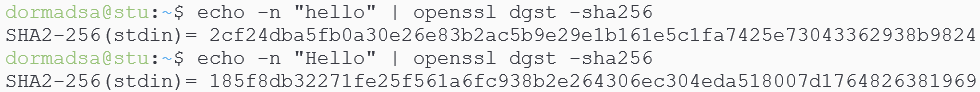
\includegraphics[width=0.9\textwidth]{figures/algos/hash-differences.png}}
  \caption{Two strings, "hello" and "Hello" being hashed, producing two very different digests.}
  \label{fig:hashes}
\end{figure}

\subsection{Alternate Hashing Algorithms}

SHA256 is not the only option in DNSSEC for hashing the meta data. There are various other functions, like MD5, SHA1, SHA384, SHA512. 
There are various pros and cons for each hashing algorithm. For instance with SHA512, compared to the $2\textsuperscript{256}$ of SHA256, 
$2\textsuperscript{512}$ is an astronomically larger number of possible hashes, but also doubles the length overall. \href{https://www.rfc-editor.org/rfc/rfc8624#section-3.1}{RFC8624} states 
that hashing with SHA 512 is NOT RECOMMENDED, due to the increase in message size and limited added security. However, you must be able to validate with SHA512, because it is available to be used. \cite{rfc8624}


\subsection{Signing with RSA}

My algorithm of choice for the signing half of the signatures is RSA. The two keys, the KSK being 2048 bits and the ZSK being 1024 bits, differ in size because the KSK is important and gets used less frequently than the ZSK.
RSA is a solid option for keys as of now, they are still very difficult and infeasible 
to crack, especially with a bigger key size. However, with the rise of quantum computing, changes may have to be made.


In the environment, I am manually signing these records with the private key pulled straight from the server myself, and then using the public key to verify the signatures. This is a good way to test the validation process, because I 
can control the data that is being signed and verified. Not only that, but I am also creating the signature myself to prove that the received signature is valid as well.

\subsection{Alternate Signing Algorithms}

Some alternative algorithms that could be used for signing are DSA (Digital Signature Algorithm), ECDSA (Elliptic Curve Digital Signature Algorithm), Ed25519. However, ECDSA provides the same if not better security as RSA with smaller key size. 
ECDSA signatures are much smaller than RSA signature, roughly half to a quarter of the size in some cases. This algorithm is also generally faster when signing, but potentially slower when verifying compared to RSA. The math is also very complex 
and less intuitive with this algorithm, compared to the more known RSA.\cite{ecdsa} 
A great site showing more information about the comparison between DNSSEC algorithms is \href{https://oneuptime.com/blog/post/2026-01-15-choose-dnssec-algorithm-rsa-ecdsa/view}{here}. 
More information on both hashing and signing algorithms and their compatibility with DNSSEC can be found at \href{https://www.rfc-editor.org/rfc/rfc8624#section-3.1}{RFC8624}.


% Both from BASE64 and the DNSSEC key to .pem
% \subsection{Alternative Key Encoding} 

% In order to use the keys generated in my lab environment, I had to convert them from the format that they were generated in to a format that could be used in my C code. The keys were 
% generated in the DNSSEC format, which had extra information and wasn't formatted correctly, so I needed to convert them to PEM format to use in my code.

\section{RRSIG Construction}
% Talk about how I built the data manually, how it could be done more dynamically in the future through code.
To build the RRSIG records, I followed the format laid out in \hyperref[subsec:rrsig]{Resource Record Signature}. I read in the data from a file, which was pulled from Wireshark captures, 
and then built the RRSIG record according to the format. First, the RRSIG metadata is built, which includes the type of record, the algorithm used, the labels, the original TTL, the signature 
expiration and inception times, the key tag, and the signer's name. Then, the canonicalized RRSet is appended to the data, and the sigbase is completed. Pictured below in 
\cref{fig:rrsig-metadata} is the general layout for the data to be hashed. In this image, the record type is an A record, and the rest of the data is filled in with the appropriate values for the record being signed.\cite{rfc4034}

\begin{figure}[htbp]
  \centering
  \fbox{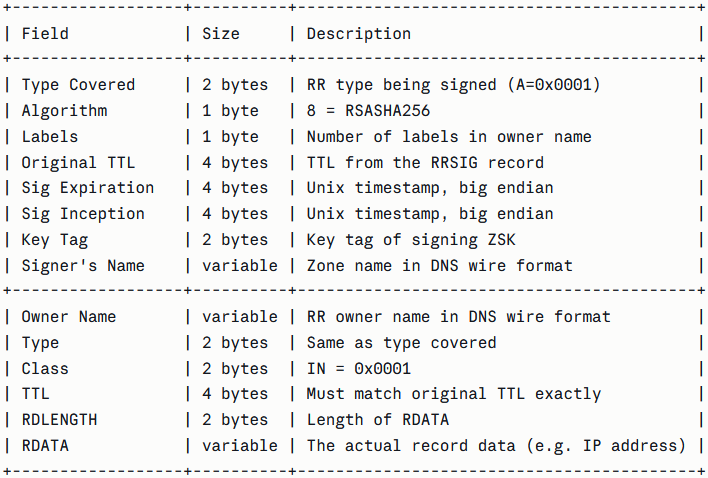
\includegraphics[width=0.8\textwidth]{figures/algos/rrsig-metadata.png}}
  \caption{A diagram of how the data is laid out and then hashed for signatures, generated by Claude.}
  \label{fig:rrsig-metadata}
\end{figure}

\subsection{Importance Of Canonicalization}

Canonicalization is critical to the DNSSEC process because it is a deterministic way to order data, leading to signatures being able to be uniform across different implementations. 
If the data is not canonicalized, then the signatures may not be valid across different implementations, because the data may be ordered differently. Any variation, even the slightest change, 
can lead to a completely different resulting signature.

\section{OpenSSL}

For this project, I used OpenSSL behind the scenes with the tools I ran in the previous section. OpenSSL is a powerful library that provides various cryptographic 
functions, including those needed for DNSSEC signing. It allows me to generate keys, create signatures, and manage certificates, which are essential components of the DNSSEC infrastructure. 
OpenSSL even provides support for converting data from Base64 into binary.

When I run the \texttt{dnssec-signzone} command, it utilizes OpenSSL to perform the cryptographic operations required for signing the zone file. By doing this, 
it hashes the data and then signs it with the private key in the background.

To complete the signing process, OpenSSL provides a function called EVP\_DigestSign, which allows me to create a signature using the specified hashing algorithm and private key. This function 
takes care of the details of the signing process, making it easier for me to implement DNSSEC signing in my code. Rather than having to separately hash and then sign the data, this function takes care of both.
It hashes the raw data, computes the digest, pads it, and then signs it with the private key.\cite{evp-sign}

\section{Performance Considerations}

Compared ti Regular DNS, DNSSEC has much more overhead and computational actions going on in the background. Not only does the packet size greatly increase in general, but also the signing 
and verification process adds a lot of overhead. The signing process involves hashing the data and then signing it with the private key, which can be computationally expensive, especially for 
larger zones. The verification process also involves hashing the data and then verifying the signature with the public key, which can also be computationally expensive. However, the added 
security provided by DNSSEC is worth the performance tradeoff, as it helps to protect against various attacks on DNS, such as cache poisoning and spoofing, is wel worth these performance considerations.\cite{bind-9}